\documentclass{beamer}
\mode<presentation>
{
	%\usetheme{CambridgeUS}
	\usetheme{Madrid}
	\usecolortheme{default}
	\usefonttheme{serif}
}
\usepackage[utf8]{inputenc}
\usepackage[russian]{babel}
\usepackage{cmap}
\usepackage{listings}
\usepackage{lmodern}
\usepackage{color}
% нафиг нужен minted?
%\usepackage{minted}

\definecolor{links}{HTML}{2A1B81}
\hypersetup{colorlinks,linkcolor=,urlcolor=links}

\begin{document}
\title
[GlusterFS]
{GlusterFS}
\author
[Подкопаев Антон, Алексеев Антон]
{
Подкопаев Антон, \texttt podkoav239@gmail.com\\
\and
Алексеев Антон, \texttt anton.m.alexeyev@gmail.com
}
\institute[Computer Science Center]{Computer Science Center}
\date [14-03-13]{14 марта 2013}

\begin{frame}[plain]
	\titlepage
\end{frame}

\begin{frame}{Распределенные файловые системы}
	\begin{itemize}
		\item Доступ с многих хостов
		
		\item Инкапсуляция расположения файлов
		% A consistent name space exists encompassing local as well as remote files. The name of a file does not give its location.
		
		\item Реплики и отказоустойчивость
		% That is, when a limited number of nodes in a file system go offline, the system continues to work without any data loss.
		
		\item Параллельный доступ
		% All clients have the same view of the state of the file system. This means that if one process is modifying a file, any other processes on the same system or remote systems that are accessing the files will see the modifications in a coherent manner.
		
		\item Масштабируемость
		% The file system should work well in small environments (1 machine, a dozen machines) and also scale gracefully to huge ones (hundreds through tens of thousands of systems).

		%\item MapReduce
	\end{itemize}
\end{frame}

\begin{frame}{Распределенные файловые системы. Основные компоненты}
	\begin{itemize}
		\item Клиент
		\item Сервер данных
		\item Сервер метаданных
	\end{itemize}
	\pause
	GlusterFS:

	Сервер данных в том числе выполняет и функции сервера метаданных
\end{frame}

\begin{frame}{GlusterFS}
	\begin{itemize}
		% \item Network/cluster filesystem written in user space
		% \item Scale up to petabytes of storage under a single mount point
		\item Сетевая фаловая система, работающая в user space
		\item До нескольких петабайт данных в одной точке монтирования
	\end{itemize}
	\begin{figure}[h]
		\centering
		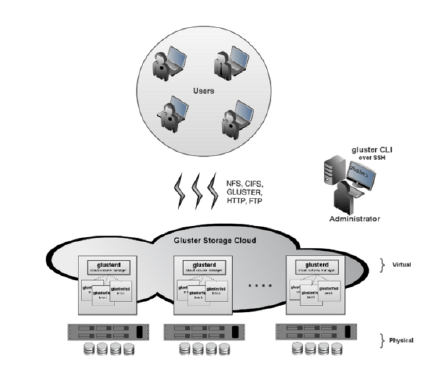
\includegraphics[width=0.7\linewidth]{scheme.png}
	\end{figure}
% GlusterFS is a powerful network/cluster filesystem written in user space which uses FUSE to hook itself with VFS layer.
% GlusterFS takes a layered approach to the file system, where features are added/removed as per the requirement.
% Though GlusterFS is a File System, it uses already tried and tested disk file systems like ext3, ext4, xfs, etc. to store the data.
% It can easily scale up to petabytes of storage which is available to user under a single mount point.
\end{frame}

\begin{frame}{Термины GlusterFS}
	\begin{itemize}
		% \item Brick     % The brick is the storage filesystem that has been assigned to a volume.
		% \item Subvolume % A brick after being processed by at least one translator.
		% \item Volume    % The final share after it passes through all the translators.

		\item Brick           % The brick is the storage filesystem that has been assigned to a volume.
		\item Логический диск % The final share after it passes through all the translators.

		%\item Client
		% The machine which mounts the volume (this may also be a server).
		%\item Server
		% The machine (virtual or bare metal) which hosts the actual filesystem in which data will be stored.

		% \item Translator
		% The brick's first translator (or last, depending on what direction data is flowing) is the storage/posix translator that manages the direct filesystem interface for the rest of the translators.
		% The configuration of translators (since GlusterFS 3.1) is managed through the gluster command line interface (cli), so you don't need to know in what order to graph the translators together.
		% All the translators hooked together to perform a function is called a graph. 		

		% \item Trusted storage pool
		\item Доверенные хранилища
		% Before you can configure a GlusterFS volume, you must create a trusted storage pool consisting of the
		% storage servers that provides bricks to a volume.
		% A storage pool is a trusted network of storage servers. 
	\end{itemize}
\end{frame}

\begin{frame}{Типы логических дисков}
	\begin{itemize}
		\item Распределеные
		\item Реплицируемые
		\item Разделяющие
		\vspace{1cm}
		\item Распределенные разделяющие
		\item Распределенные реплицируемые
		\item Разделяющие реплицируемые
	\end{itemize}
\end{frame}

\begin{frame}{Распределенные логические диски (1)}
	\begin{figure}[h]
		\centering
		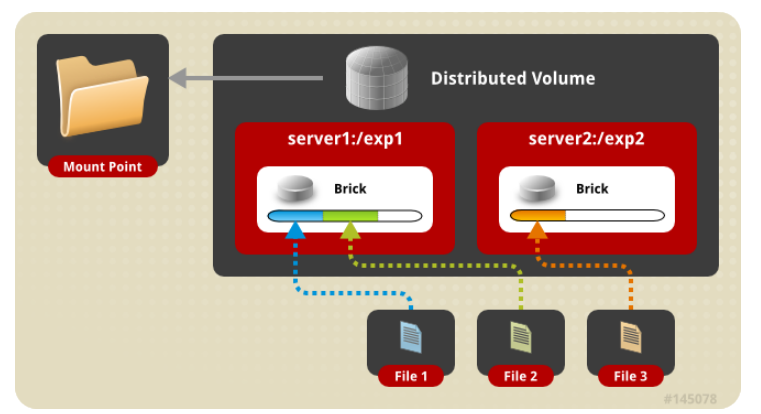
\includegraphics[width=0.8\linewidth]{distributed.png}
	\end{figure}
	% \begin{block}{}
		% gluster volume create test-volume server1:/exp1 server2:/exp2
	% \end{block}

	% The server that the files are written to is calculated by hashing the filename.
	% If the filename changes, a pointer file is written to the server that the new hash
	% code would point to, telling the distribute translator which server the file is actually on.
\end{frame}

\begin{frame}{Распределенные логические диски (2)}
	\begin{block}{Плюсы}
		\begin{itemize}
			% \item More servers - better scaling
			\item Больше серверов => выше производительность при параллельном доступе
			% in terms of random file access. As long as clients aren't all retrieving the same file,
			% their access should be spread pretty evenly across all the servers.

			% \item Increasing volume - adding a new server % on-the-fly
			\item Увеличение диска = добавление сервера (можно во время работы) % on-the-fly
		\end{itemize}
	\end{block}
	\begin{block}{Минусы}
		\begin{itemize}
			\item Потеря сервера = потеря данных на нем
			\item Файл не может быть больше размера узла
			\item Смена имени файла => дополнительное время на lookup
		\end{itemize}
	\end{block}
\end{frame}

\begin{frame}{Реплицируемые логические диски}
	\begin{figure}[h]
		\centering
		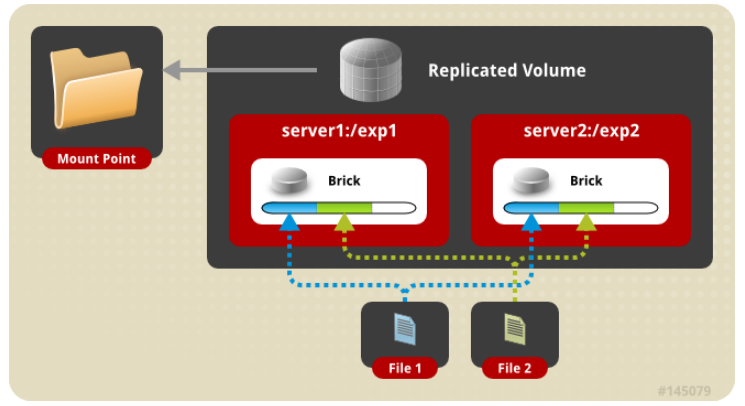
\includegraphics[width=0.8\linewidth]{replicated.png}
	\end{figure}
	% \begin{block}{}
	% 	gluster volume create test-volume replica 2 server1:/exp1 server2:/exp2
	% \end{block}
\end{frame}

\begin{frame}{Разделяющие логические диски}
	\begin{figure}[h]
		\centering
		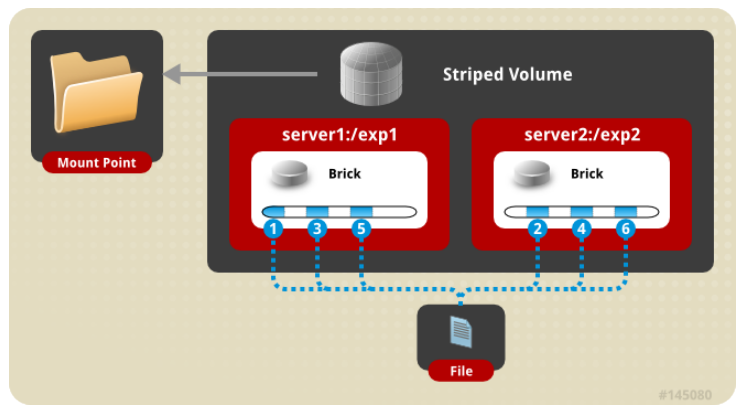
\includegraphics[width=0.8\linewidth]{striped.png}
	\end{figure}
	% \begin{block}{}
	% 	gluster volume create test-volume stripe 2 server1:/exp1 server2:/exp2
	% \end{block}
\end{frame}

\begin{frame}{Запуск GlusterFS (1)}
	\begin{block}{}
		\inputminted{bash}{sc2}
	\end{block}
	\pause
	\begin{block}{}
		\inputminted{bash}{sc1}
	\end{block}
	\pause
	\begin{block}{}
		\inputminted{bash}{sc3}
	\end{block}
\end{frame}

\begin{frame}{Запуск GlusterFS (2)}
	\begin{block}{Распределенные}
		\$gluster volume create test-volume server1:/exp1 server2:/exp2
	\end{block}
	\begin{block}{Реплицируемые}
		\$gluster volume create test-volume replica 2 server1:/exp1 server2:/exp2
	\end{block}
	\begin{block}{Разделяющие}
		\$gluster volume create test-volume stripe 2 server1:/exp1 server2:/exp2
	\end{block}
\end{frame}

\begin{frame}{Добавление серверов}
	\begin{block}{} 
		\$gluster peer probe new\_server

		\pause
		\$gluster volume add-brick vol\_name new\_brick

		\pause
		\$gluster volume info
	\end{block}
	\pause
	\vspace{1cm}
	Для расширения реплицируемых (разделяющих) дисков надо добавлять количество серверов, кратное фактору реплики (разбиения)
\end{frame}

\begin{frame}{Удаление серверов}
	\begin{block}{} 
		\$gluster volume remove-brick vol\_name new\_brick start

		\pause
		\$gluster volume remove-brick vol\_name new\_brick status

		\pause
		\$gluster volume remove-brick vol\_name new\_brick commit
	\end{block}
\end{frame}

\begin{frame}{Рычажки}
	\begin{block}{Все настройки осуществляются так}
		 \$gluster volume set vol\_name option param	
	\end{block}
	\begin{block}{Пример}
		 \$gluster volume set myvolume performance.cache-size 256MB	
	\end{block}
\end{frame}

\begin{frame}{Рычажки}
	\begin{block}{}
		\begin{tabular}{ p{6cm} p{5cm} }
			\textbf{auth.allow} & IP-адреса клиентов, с джокерами: 192.168.1.\* \\
			\textbf{auth.reject} &  IP-адреса заблокированных клиентов \\
			\textbf{client.grace-timeout} & время жизни замков, поставленных клиентом, после разрыва соединения, в секундах (10--1800) \\
			\textbf{cluster.self-heal-window-size} & максимальное число блоков в файле, для которых self-heal происходит одновременно (0-1025)\\
		\end{tabular}
	\end{block}
\end{frame}

\begin{frame}{Рычажки}
	\begin{block}{}
		\begin{tabular}{ p{6cm} p{5cm} }
			\textbf{cluster.data-self-heal-algorithm} & тип self-heal: full (копирование всего файла), diff (копирование только несинхронизированных блоков), reset (если файла нет --- полное копирование, если размер файла близок к размеру страницы диска --- чтение несколькими операциями) \\
		\end{tabular}
	\end{block}
\end{frame}


\begin{frame}{Рычажки}
	\begin{block}{}
		\begin{tabular}{ p{6cm} p{5cm} }
			\textbf{cluster.min-free-disk} & сколько процентов диска должны оставаться незанятыми \\ % non-uniform bricks?
			\textbf{cluster.stripe-block-size} & размер страйпа (в байтах) \\
			\textbf{cluster.self-heal-daemon} & включение / выключение фонового self-heal на репликах (on/off) \\
			\textbf{diagnostics.brick-log-level} & уровень логов bricks: INFO, DEBUG, WARNING, ERROR, CRITICAL, NONE, TRACE \\
			\textbf{diagnostics.client-log-level} & уровень логов клиентов \\
			\textbf{diagnostic.dump-fd-stats} & статистика по операциям над файлами (on/off) \\
		\end{tabular}	
	\end{block}
\end{frame}


\begin{frame}{Рычажки}
	\begin{block}{}
		\begin{tabular}{ p{6cm} p{5cm} }
			\textbf{feature.read-only} & монтирование диска в режиме read-only для всех клиентов (on/off)\\
			\textbf{features.lock-heal} & self-healing замков при разрыве соединения (on/off)\\
			\textbf{features.quota-timeout} & объём памяти для каждой директории кэшируется; можно указать макс. допустимое время пребывания любой директории в кэше (0-3600 сек.) \\
		\end{tabular}
	\end{block}
\end{frame}


\begin{frame}{Рычажки}
	\begin{block}{}
		\begin{tabular}{ p{6cm} p{5cm} }
			\textbf{geo-replication.indexing} & автоматическая синхронизация изменений от master к slave \\
			\textbf{network.frame-timeout} & время, через которое операция объявляется <<мёртвой>>, если сервер не отвечает \\ % не понял
			\textbf{network.ping-timeout} & время ожидания клиентом ответа от сервера (default: 42 сек.!); после разрыва все данные, связанные с клиентом, уничтожаются; при восстановлении соединения --- восстановление всех ресурсов и замков. Очень, очень дорого. Не надо так делать. \\
		\end{tabular}
	\end{block}
\end{frame}

\begin{frame}{Рычажки}
	\begin{block}{}
		\begin{tabular}{ p{6cm} p{5cm} }
			\textbf{nfs.volume-access} & тип доступа для sub-volume (read-write/read-only) \\
			\textbf{nfs.trusted-write} & запрещать клиенту коммитить, если произошёл UNSTABLE write; STABLE writes --- синхронизируются (on/off) \\
			\textbf{nfs.trusted-sync} & все записи и запросы на коммит считаются асинхронными (на момент ответа не гарантируется, что запись произведена на все диски) \\
%			\textbf{nfs.export-dir} & не понял \\
%			\textbf{nfs.export-volumes} & разрешение на экспорт дисков \\
			\textbf{nfs.rpc-auth-unix} & включение аутентификации AUTH\_UNIX (default: On) \\
			\textbf{nfs.rpc-auth-null} & включение аутентификации AUTH\_NULL (default: On) \\
		\end{tabular}
	\end{block}
\end{frame}


\begin{frame}{Рычажки}
	\begin{block}{}
		\begin{tabular}{ p{6cm} p{5cm} }
			\textbf{nfs.rpc-auth-allow} & IP-адреса и hostnames, которым разрешается устанавливать соединение с сервером \\
			\textbf{nfs.rpc-auth-reject} & те, кому нельзя \\
			\textbf{nfs.ports-insecure} & разрешать соединения непривилегированным хостам (default: off) \\
%			\textbf{nfs.register-with-portmap} & отключение регистрации с помощью portmap-service \\
			\textbf{nfs.port} & для связывания Gluster NFS с недефолтным номером порта (38465--38467)\\
			\textbf{nfs.disable} & запретить экспорт диска NFS (default: off) \\
%			\textbf{performance.write-bihind-window-size} & per-file-write-behind buffer size \\
		\end{tabular}
	\end{block}
\end{frame}



\begin{frame}{Рычажки}
	\begin{block}{}
		\begin{tabular}{ p{6cm} p{5cm} }
			\textbf{performance.io-thread-count} & число потоков транслятора управляющего IO \\ %так ли?
			\textbf{performance.cache-max-file-size} & max размер кэша транслятора (до $2^{64} - 1$ байт)\\
			\textbf{performance.cache-min-file-size} & min размер кэша транслятора (от 0 байт)\\		
			\textbf{performance.cache-refresh-timeout} & интервал, с которым кэш будет обновляться (0-61 сек.) \\
			\textbf{performance.cache-size} & размер кэша чтения (default: 32 MB) \\
		\end{tabular}
	\end{block}
\end{frame}


\begin{frame}{Рычажки}
	\begin{block}{}
		\begin{tabular}{ p{6cm} p{5cm} }
			\textbf{server.allow-insecure} & разрешать соединения непривилегированным хостам (default: on) \\
			\textbf{server.grace-timeout} &  время жизни замка после разрыва связи (10--1800  сек.) \\
			\textbf{server.statedump-path} &  путь к дампу состояния системы (default: /tmp brick'а) \\		
		\end{tabular}
	\end{block}
\end{frame}

\begin{frame}{Ссылки}
	\begin{itemize}
		\item \url{http://www.gluster.org/}
		\item Взрослеем с GlusterFS \url{http://habrahabr.ru/post/140031/}
		\item GlusterFS, опыт новой версии \url{http://habrahabr.ru/post/157029/}
	\end{itemize}
\end{frame}

\end{document}
